\chapter{\SOA\ (SOA)}
\label{chap:soa}
Der Begriff "'Service-orientierte Architektur (kurz SOA)"' ist nicht eindeutig definiert. Je nachdem welche Person in einem Unternehmen man fragt, erhält man unter Umständen eine komplett andere Definition. \frqq Die Meisten Definitionen stimmen jedoch zum größten Teil überein und stehen nicht im Konflikt mit einander.\flqq\cite[vgl. Seite 6]{100QA}

Für einen Kaufmann ist SOA etwas anderes als für einen Analysten, damit SOA jedoch verstanden werden kann, werden zunächst einmal einige Definitionen nach \cite{100QA}\ genannt:
\begin{enumerate}
       \item \frqq To the chief information officer (CIO), SOA is a journey that
       promises to reduce the lifetime cost of the application portfolio [...].\flqq \cite[vgl. Seite 6]{100QA}
    
       \item \frqq To the business executive, SOA is a set of services that can be exposed to their customers, partners, and other parts of the organization. Business capabilities, function, and business logic can be combined and recombined to serve the needs of the business now and tomorrow. Applications serve the business because they are composed
       of services that can be quickly modified or redeployed in new
       business contexts, allowing the business to quickly respond to changing
       customer needs, business opportunities, and market conditions.\flqq \cite[vgl. Seite 6]{100QA}
       
       \item \frqq To the business analyst, SOA is a way of unlocking value, because business processes are no longer locked in application silos. Applications no longer operate as inhibitors to changing business needs.\flqq \cite[vgl. Seite 6]{100QA}
       
       \item \frqq To the chief architect or enterprise architect, SOA is a means to
       create dynamic, highly configurable and collaborative applications
       built for change. SOA reduces IT complexity and rigidity. SOA becomes the solution to stop the gradual entropy that makes applications
       brittle and difficult to change. SOA reduces lead times and costs
       because reduced complexity makes modifying and testing applications
       easier when they are structured using services.\flqq \cite[vgl. Seite ]{100QA}
\end{enumerate}
Jeder der genannten Rollen hat eine eigene klare Definition von dem was Service-orientierte Architektur ist. Jeder der Definitionen ist jedoch nur ein Teil dessen für was SOA verwendet werden kann.

\section{Grundlagen}
\label{sec:Grundlagen}
Bevor jedoch damit angefangen werden kann SOA in ein Unternehmen einzuführen, muss zunächst einmal geklärt werden, welches Ziel hinter \SOA en stehen. Zunächst einmal sei erwähnt, das SOA nicht das Ziel hat die Entwicklung zu vereinfachen oder voran zu bringen. SOA soll die Unternehmensweiten Geschäftsprozesse optimieren und eine Wertschöpfungskette erzeugen.

\subsection{Unternehmens Komponenten}
\label{subsec:UnternehmensKomponenten}
Dazu müssen zunächst einmal alle Komponenten eines Unternehmens identifiziert werden. Die nachstehende Abbildung (\ref{fig:UnternehmensKomponenten}) zeigt ein Beispiel dieser Identifizierung:

\begin{figure}[htb]
    \centering 
    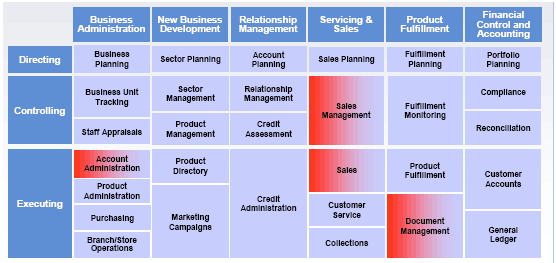
\includegraphics[width=\linewidth]{content/images/UnternehmensKomponenten}\
    \quelle\url{http://www.jot.fm/issues/issue_2008_05/column5/}
    \caption[Unternehmens Komponenten]{Unternehmens Komponenten\\}
    \label{fig:UnternehmensKomponenten}  
\end{figure} 
\newpage
Aus diesen Komponenten müssen nun die Geschäftsprozesse identifiziert werden. Daraus ergeben sich anschließend die Komponenten, welche unter einander kommunizieren müssen. Die in der Abbildung Rot dargestellten Komponenten sind schließlich das Resultat aus der Analyse.

\subsection{Wertschöpfungskette}
\label{subsec:Wertschoepfungskette}
\frqq Die Wertschöpfungskette stellt die zusammenhängenden Unternehmensaktivitäten des betrieblichen Gütererstellungsprozesses grafisch dar.\flqq \cite{gabler}

SOA soll dabei helfen die Wertschöpfungskette sowohl darzustellen, als auch sie zu verwalten und damit zu optimieren. In Abbildung \ref{fig:UnternehmensKomponenten} sind die zentralen Komponente eines Geschäftsprozesses rot markiert. Mit Hilfe von SOA werden aus diesen Komponenten eine Wertschöpfungskette gebildet.

\section{Architektur}
\label{sec:SoaArchitektur}
Aus der oben dargestellten Auflistung können verschiedene Definitionen für Service-orientierte Architekturen entnommen werden. Die Architektur kommt der 3. Definition schon ziemlich nahe. Genauso wie Microservices sind auch die Services innerhalb einer Service-orientierten Architektur eigenständig und sollen nur eine Aufgabe erledigen. Anders als bei einem Microservice-System jedoch, bei dem die einzelnen Services untereinander kommunizieren dürfen, ist in einem SOA-System die Kommunikation zwischen einzelnen Services untersagt.

Die Abbildung der Geschäftsprozesse erfolgt in einem sogenannten Enterprise-Service-Bus (Kurz ESB), welcher die einzelnen Services Orchestriert (siehe Abbildung \ref{fig:ServiceOrchestration}).

\subsection{Orchestration}
\label{subsec:orchestration}
Bei der Orchestration handelt es sich um eine Komposition von Services. Ein Geschäftsprozess wird zwar mit Hilfe von mehreren Services abgebildet, jedoch ist nur ein Service dafür zuständig den Geschäftsprozess durchzuführen.
\newpage
\begin{figure}[htb]
    \centering 
    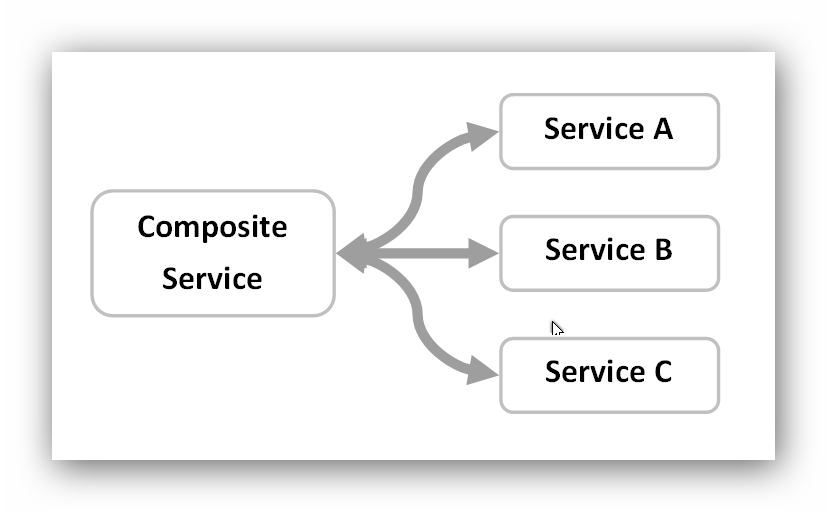
\includegraphics[width=\linewidth]{content/images/ServiceOrchestration}\
    \caption[Orchestration]{Orchestration}
    \label{fig:ServiceOrchestration}  
\end{figure}
\noindent
Wie die Abbildung zeigt besteht \textbf{\underline{keine}} Verbindung zwischen:
\begin{itemize}
    \item A \& B
    \item A \& C
    \item B \& C
\end{itemize}
Nur der "`Composite Service"' nutzt die anderen Services, um den Geschäftsprozess abzubilden. Diese Art der Kommunikation nennt man Orchestration.

\subsection{Choreographie}
\label{subsec:choreographie}
Anders als bei der Orchestration können Services bei der Choreographie beliebig untereinander kommunizieren. Das ist vor allem dann Sinnvoll, wenn verschiedene Service andere Service über Änderungen oder andere Aktionen informieren müssen.

\begin{figure}[htb]
    \centering 
    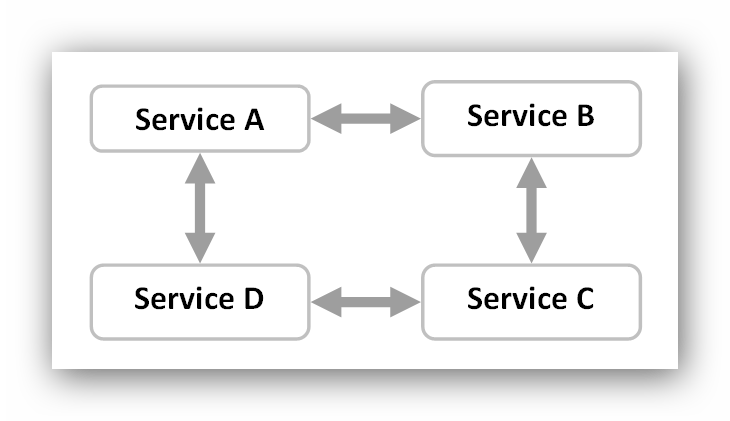
\includegraphics[width=\linewidth]{content/images/ServiceChoreography}\
    \caption[Choreographie]{Choreographie}
    \label{fig:ServiceOrchestration}  
\end{figure}

Wie bereits oben erwähnt ist der Enterprise Service Bus die zentrale Einheit bei der Service-orientierten Architektur (SOA) über die alle Kommunikation läuft und welcher die Geschäftsprozesse abbildet. Daher ist eine Choreographie unter den Services in diesem Architekturmodell nicht möglich.

\section{Enterprise Service Bus - ESB}
\label{sec:esb}
Der \textit{Enterprise Service Bus} ist die zentrale Einheit in einem SOA-System. Am einfachsten lässt sich das an einem Beispiel erklären.
\\
Man Stelle sich eine Banking-Anwendung vor, an der man sich anmeldet. Es werden daraufhin folgende Informationen angezeigt:

\begin{enumerate}
    \item Name
    \item Kontostand
    \item EC- und Kreditkarten
    \item Liste der Aktienfonds
\end{enumerate}

Jede Information stammt aus einem anderen Teil des Systems und werden von verschiedenen Anwendungen über Schnittstellen bereitgestellt. Die Schnittstellen können sich dabei von Anwendung zu Anwendung unterscheiden. So kann zum Beispiel eine Anwendung die Informationen über HTTP bereitstellen, während eine andere sie über SOAP bereitstellt. So können die Informationen zum Beispiel aus einem CRM-System (Kundenbeziehungsmanagement-System) stammen oder durch PHP oder Ruby erzeugt werden.

Anders als man jedoch vermuten würde, lässt man die Oberfläche, bzw. das System, nicht direkt mit den einzelnen Komponenten reden. Die gesamte Kommunikation läuft dabei über den \textit{Enterprise Service Bus} ab. Nachstehende Abbildung soll dies genauer erläutern:

\begin{figure}[htb]
    \centering 
    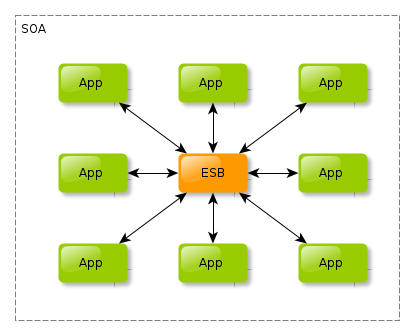
\includegraphics[width=\linewidth]{content/images/esb-ok}\
    \caption[ESB]{Enterprise Service Bus}
    \quelle\url{https://zato.io/docs/intro/esb-soa-de.html}
    \label{fig:esb}  
\end{figure}
\newpage
Benötigt eine Anwendung (in der Abbildung App genannt) Informationen, konsultiert diese zunächst den ESB. Der ESB kennt die anderen Anwendungen und stellt daraufhin die angeforderten Informationen bereit.